%!Tex Root = ../Main.tex
% ./Packete_und_Deklarationen.tex

\chapter{Implementierung}
\label{ch:implementierung}
\section{Architektur}
% Unterscheid zur Architektur aus dem Bachelorprojekt

% Cross Compiler
\begin{figure}[H]
  \centering
  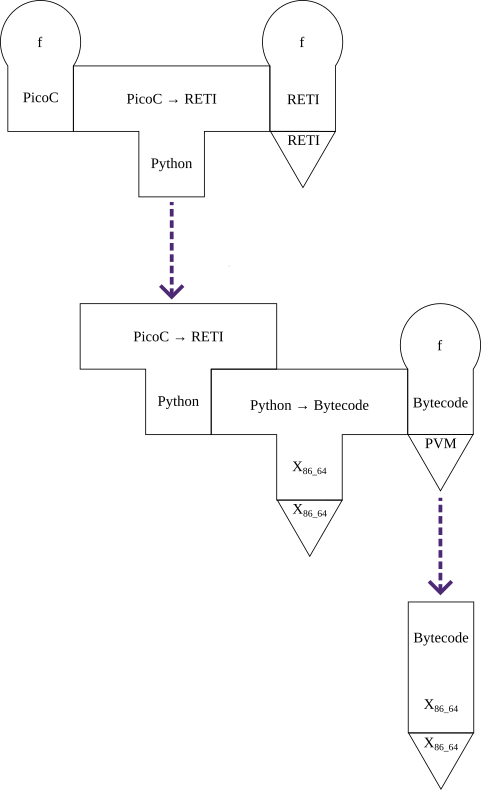
\includegraphics[width=0.5\linewidth]{./figures/summarized_cross_compiler.png}
  \caption{Cross-Compiler Kompiliervorgang ausgeschrieben}
\end{figure}

\begin{figure}[H]
  \centering
  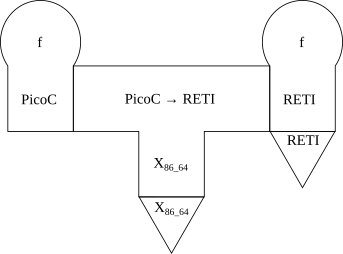
\includegraphics[width=0.33\linewidth]{./figures/compiliervorang_mit_machiene.png}
  \caption{Cross-Compiler Kompiliervorgang Kurzform}
\end{figure}

\begin{figure}[H]
  \centering
  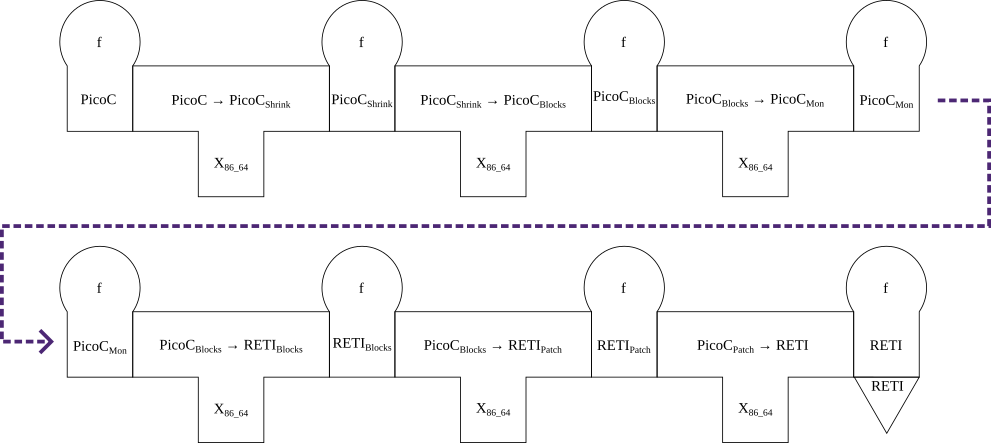
\includegraphics[width=\linewidth]{./figures/passes.png}
  \caption{Architektur mit allen Passes ausgeschrieben}
\end{figure}

\section{Lexikalische Analyse}
\subsection{Verwendung von Lark}
% erwähnen, dass in Lark die Grammatiken L_Lex und L_Parse gemischt sind
% EBNF erwähnen
% (erwähnen, dass finalle Grammatik im Appendix)
\subsection{Basic Parser}
\section{Syntaktische Analyse}
\subsection{Verwendung von Lark}
% Vorteile von Lark
\subsection{Umsetzung von Präzidenz}
Die \colorbold{PicoC Sprache} hat dieselben \colorbold{Präzidenzregeln} implementiert, wie die \colorbold{Sprache C} \footcite{noauthor_c_nodate}. Die \colorbold{Präzidenzregeln} von \colorbold{PicoC} sind in Tabelle~\ref{tab:reference_table} aufgelistet.

\begin{table}[H]
  \center
  \begin{tabulary}{\linewidth}{|C|C|L|L|}
  \toprule
  \colorbold{Präzidenz} &	\colorbold{Operator} & \colorbold{Beschreibung} &	\colorbold{Assoziativität} \\
  \midrule
  1	& \verb|a()|	& Funktionsaufruf & \multirow{2}{=}{Links, dann rechts $\rightarrow$} \\
    & \verb|a[]|	& Indexzugriff & \\
    & \verb|a.b| & Attributzugriff & \\
  \hline
  2	&	\verb|-a| & Unäres Minus & \multirow{2}{=}{Rechts, dann links $\leftarrow$} \\
    & \smalltt{!a $\thicksim$a}	& Logisches NOT und Bitweise NOT & \\
    & \verb|*a &a| & Dereferenz und Referenz, auch Adresse-von & \\
  \hline
  3	& \smalltt{a*b a/b a\%b} &	Multiplikation, Division und Modulo & Links, dann rechts $\rightarrow$ \\
  \cline{1-3}
  4	& \verb|a+b a-b|	& Addition und Subtraktion & \\
  \cline{1-3}
  5	& \verb|a<b a<=b| \verb|a>b a>=b| & Kleiner, Kleiner Gleich, Größer, Größer gleich & \\
  \cline{1-3}
  6 &	\verb|a==b a!=b| & Gleichheit und Ungleichheit & \\
  \cline{1-3}
  7 &	\verb|a&b| & Bitweise UND & \\
  \cline{1-3}
  8 &	\verb|a^b| & Bitweise XOR (exclusive or) & \\
  \cline{1-3}
  9 & \smalltt{a$\mid$b} & Bitweise ODER (inclusive or) & \\
  \cline{1-3}
  10	& \verb|a&&b| &	Logiches UND & \\
  \cline{1-3}
  11	& $a{\mid\mid} b$	& Logisches ODER & \\
  \hline
  12 & \verb|a=b| & Zuweisung & Rechts, dann links $\leftarrow$ \\
  \hline
  13 &	\verb|a,b|& Komma	& Links, dann rechts $\rightarrow$ \\
  \bottomrule
\end{tabulary}
\label{tab:reference_table}
\caption{Präzidenzregeln von PicoC}
\end{table}
% erwähnen von Mehrdeutigkeit und Assoziativität
% finalle Grammatik im Appendix
% Crafting Compilers Quelle benennen
\subsection{Derivation Tree Generierung}
\subsection{Early Parser}
\subsection{Derivation Tree Vereinfachung}
% Visitor erwähnen
\subsection{Abstrakt Syntax Tree Generierung}
\subsubsection{ASTNode}
\subsubsection{PicoC Nodes}
% Tabelle aller PicoC Nodes
% möglichst kurze und leicht verständliche Bezeichner für Nodes
\subsubsection{RETI Nodes}
% Tabelle aller RETI Nodes
% Transformer erwähnen
\section{Code Generierung}
\subsection{Passes}
\subsubsection{PicoC-Shrink Pass}
% dieser Pass wurde wegen
\subsubsection{PicoC-Blocks Pass}
\subsubsection{PicoC-Mon Pass}
\begin{Definition}{Symboltabelle}{symboltabelle}
\end{Definition}
\subsubsection{RETI-Blocks Pass}
\subsubsection{RETI-Patch Pass}
\subsubsection{RETI Pass}
% TODO: zusammenfassendes Bild
\subsection{Umsetzung von Pointern}
\subsection{Umsetzung von Arrays}
\subsubsection{Initialisierung von Arrays}
% kleines Extra
\subsubsection{Zugriff auf Arrayindex}
Der Zugriff auf einen bestimmten  Index eines Arrays ist wie folgt umgesetzt:

\begin{minipage}{0.4\textwidth}
  \lipsum[1-2]
\end{minipage}
\hfill
\begin{minipage}{0.6\textwidth}
  \raggedleft
  \treebox[title=PicoC Code, remember as=array_access_picoc_code, width=0.6\textwidth, breakable]{./code_examples/example_array_access.picoc}
  \vspace{0.5cm}
  \treebox[title=Abstract Syntax Tree, remember as=array_access_ast, width=0.6\textwidth, breakable]{./code_examples/example_array_access.ast}
\end{minipage}
  \treebox[title=PicoC Blocks, remember as=array_access_picoc_blocks, width=0.6\linewidth, breakable]{./code_examples/example_array_access.picoc_blocks}
  % \treebox[title=PicoC Mon, remember as=array_access_picoc_mon, width=0.6\linewidth, nobeforeafter]{./code_examples/example_array_access.picoc_mon}
  % \treebox[title=RETI Blocks, remember as=array_access_reti_blocks, width=0.6\linewidth, nobeforeafter]{./code_examples/example_array_access.reti_blocks}
  % \treebox[title=RETI Patch, remember as=array_access_reti_patch, width=0.6\linewidth, nobeforeafter]{./code_examples/example_array_access.reti_patch}
  % \treebox[title=RETI, remember as=array_access_reti, width=0.6\linewidth, nobeforeafter]{./code_examples/example_array_access.reti}
  % \caption{Veranschaulichung des Kompiliervorgangs für den Zugriff auf einen Arrayindex}
  % \label{fig:zugriff_auf_einen_arrayindex}
% TODO: extra untersciedliche Darstellungsweise gewählt für DT und AST

\subsubsection{Zuweisung an Arrayindex}
\subsection{Umsetzung von Structs}
\subsubsection{Initialisierung von Structs}
\subsubsection{Zugriff auf Structattribut}
\subsubsection{Zuweisung an Structattribut}
\subsection{Umsetzung von Funktionen}
\subsubsection{Sprung zur Main Funktion}
\subsubsection{Funktionsdeklaration und -definition}
\subsubsection{Funktionsaufruf}
\subsection{Umsetzung kleinerer Details}
% langen Sprüngen, großen Konstanten, Division durch 0
\section{Fehlermeldungen}
\subsection{Error Handler}
\subsection{Arten von Fehlermeldungen}
\subsubsection{Syntaxfehler}
\subsubsection{Laufzeitfehler}
% Fehlermeldung ist, wenn der Lexer (partielle Funktion) oder Parser nicht matcht
% Token und Nodes enthalten Position, im Transformer wird die Position von den Token auf die Nodes übertragen und auch die Symboltabelle speichert Position
